\section{Qualitätsmanagement der Informationsprozesse - MB}
\textit{Autor: Miriam Börger}


Im Folgenden wird der Qualitätsmanagement-Prozess in seinen Grundzügen definiert, am konkreten Beispiel der Minimierung von Durchlaufzeiten genauer betrachtet und praktisch mit Hilfe der IT Balanced Scorecard durchexerziert. 
Abschließend wird erörtert, welche Besonderheiten hierbei an Hochschulen bestehen und Möglichkeiten aufgezeigt, diese Schwierigkeiten zu umgehen.

\subsection{Aufgaben des Qualitätsmanagements}
In einem Informationsmanagement bildet das Qualitätsmanagement der Informationsprozesse einen zentralen Aufgabenbereich. Es übernimmt die Planung, Koordination und Steuerung der Informationsflüsse und prüft fortwährend, inwieweit eine Nutzbarkeit und Effizienz der Prozesse in der Realität gewährleistet ist, um deren Qualität gegebenenfalls mit gezielten Maßnahmen zu optimieren.\footnote{\cite{schroder_wertorientiertes_2005}}

Hierzu fungiert ein Team von Qualitätsmanagern als Vermittler zwischen den verschiedenen Parteien im Unternehmen und überbrückt potentiell auftretende Kommunikations- oder Kulturbarrieren, um eine zielorientierte und effiziente Informationsversorgung der beteiligten Parteien zu ermöglichen.

Zu Beginn des Qualitätsmanagement-Prozesses gilt es, eine Leitstrategie aufzustellen. Hierfür wird der aktuelle Ist-Zustand des Unternehmens in Bezug auf seine Organisation von Informationsflüssen analysiert. Dabei zum Vorschein kommende Schwachstellen werden erfasst und durch mögliche optimierende Handlungsoptionen ergänzt.\footnote{\cite{helmke_management_2013}}

Während der Durchführung der neu erschaffenen Maßnahmen ist das Qualitätsmanagement-Team mit der stetigen Überwachung dieser betraut. 
Bereits bei kleinen Abweichungen vom Plan kann mit gegensteuernden Maßnahmen eingegriffen werden. 
Eine im Voraus aufgestellte Zeitplanung ist hierbei ebenso wichtig wie eine klare Definition der Zuständigkeiten im Qualitätsmanagement-Team, um eine termingerechte Erreichung der gesetzten Ziele noch zu garantieren.

Nach Ablauf des gesetzten Zeitrahmens oder nach Beendigung der Maßnahmen ist es erforderlich, mittels einer sogenannten Feedback-Analyse festzustellen, inwieweit das gesteckte Ziel erreicht wurde und aus welchen Gründen es nicht zu 100\% zufriedenstellenden Ergebnissen kommen konnte. 
Die hieraus resultierenden Erkenntnisse bilden daraufhin die Grundlage für eine anschließende Feedforward-Analyse, die die weitergehend erforderlichen Maßnahmen feststeckt, um in einer weiteren Phase die Zielerreichung durch verbesserte Maßnahmen zu garantieren.\footnote{\cite{gadatsch_it-controlling_2012}}

\subsection{Prozessoptimierung durch Minimierung der Durchlaufzeiten}
Essenzielles Ziel des Qualitätsmanagement-Teams ist es, anhand bewährter Vorgehensweisen die Durchlaufzeiten von Informationen zu minimieren. 
Hierdurch wird der Informationsfluss quantitativ und qualitativ verbessert, da bestehende Abhängigkeiten der Parteien in Bezug auf die Informationen schneller bedient werden können und somit durch minimierte Wartezeiten eine beträchtliche Budgetersparnis resultiert.

\begin{figure}[h!]
	\centering
	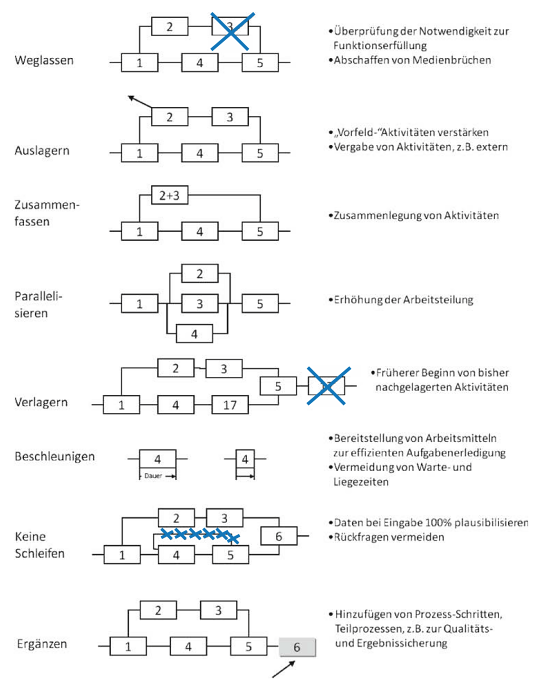
\includegraphics[width=10cm]{kapitel/gruppe1_1/bilder/minimierung_durchlaufzeiten}
	\caption{Minimierung von Durchlaufzeiten, nach Bleicher 1991, 196}
	\label{fig_minimierung_durchlaufzeiten}
\end{figure}

Wie in Abbildung \ref{fig_minimierung_durchlaufzeiten} erkennbar, existieren elementare Methoden zur Reduktion von Durchlaufzeiten nach Bleicher aus dem Jahre 1991, die noch heute ihre Gültigkeit in der Anwendung haben.\footnote{\cite{bleicher_organisation_1991}}

Insbesondere das Zusammenfassen von Aktivitäten hat den entscheidenden Vorteil, dass Abstimmungsprozesse und Abhängigkeiten zwischen mehreren Parteien entfallen und somit die Umsetzungsdauer auf ein Minimum reduziert wird. 

Auch die Methode des Parallelisierens sollte in den Fokus gerückt werden. Wie in Abbildung 1 ersichtlich, werden hierbei mehrere Parteien, die für eine darauffolgende Partei relevant sind, zeitgleich geschaltet, um Wartezeiten zu verhindern. 

Zu guter Letzt sei das Ergänzen von Prozessschritten betont. Auf den ersten Blick scheint diese Methode paradox, da durch Ergänzung weiterer Parteien der Zeit- und Arbeitsaufwand vorerst erhöht wird. Durch einen globaleren Blick wird schnell deutlich, dass ohne diese Parteien zu einem späteren Zeitpunkt Problematiken entstehen können, die in ihrer Lösung viel zeit- und arbeitsintensiver sind und das Unternehmen in seiner Prozessqualität deutlich zurückwerfen könnte.

Die in Abbildung \ref{fig_minimierung_durchlaufzeiten} gezeigten Methoden zur Durchlaufzeit-Minimierung sollten also vom Qualitätsmanagement-Team von Beginn an in die Planung mit einbezogen werden, da mit minimalem Aufwand eine weitreichende, inhaltlich und finanziell positive Auswirkung auf die Qualität des Gesamtprozesses erzeugt wird. 

\subsection{Anwendung des Qualitätsmanagements am Beispiel der IT Balanced Scorecard}
Das strategisch-operative Konzept für eine qualitative Unternehmenssteuerung aus den 90er Jahren von R. S. Kaplan und D. P. Norton hat sich im Laufe der Zeit zum Standardinstrument entwickelt.\footnote{\cite{friedag_scorecard_2004}}

Grundlegend für die IT Balanced Scorecard ist das Schema Eingabe $\to$ Verarbeitung $\to$ Ausgabe $\to$ Resultat. Die Kombination von Qualität der Mitarbeiter, Kundenorientierung und finanzielle Ziele ermöglicht die Generierung und Sicherung eines gelungenen Informationsmanagements.\footnote{\cite{gabriel_inm_2003}}

\begin{figure}[h!]
	\centering
	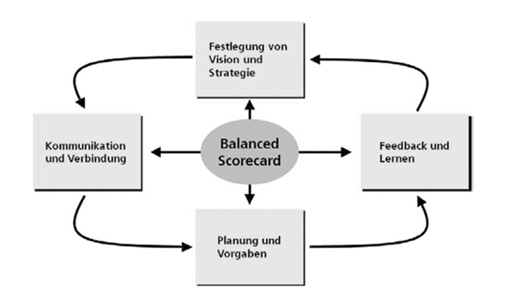
\includegraphics[width=10cm]{kapitel/gruppe1_1/bilder/balanced_scorecard}
	\caption{Balanced Scorecard Kreislauf, nach Gadatsch}
	\label{fig_balanced_scorecard_cycle}
\end{figure}

Die IT Balanced Scorecard zeichnet sich – wie in Abbildung \ref{fig_balanced_scorecard_cycle} deutlich wird – durch eine stetige Feedback- und Feedforward-Kommunikation aus. 
Zu Beginn des Managementprozesses werden in der Phase „Planung und Vorgaben“ die grundlegenden Ziele des Unternehmens definiert.

In einem nächsten Schritt werden in der Phase „Vision und Strategie“ Kernaussagen zur Strategiefindung erarbeitet, insbesondere im Hinblick auf den Zusammenhang von Ursache und Wirkung, sowie Optimierungsmöglichkeiten zusammengestellt. 

Das Handlungskonzept wird in „Feedback und Lernen“ final ausformuliert und in der vierten Phase „Kommunikation und Verbindung“ mit der Strategie und übergeordneten Zielen verknüpft.

Eine detaillierte Dokumentation von Teilzielen erhöht in dieser Phase die Motivation der Mitarbeiter zur Zielerreichung.\footnote{\cite{kaufmann_feinschliff_2002}}

Die Definition von klaren Zielen, Bedingungen und Kennzahlen generiert ein komplexes Kennzahlensystem, welches durch Herunterbrechen der Strategie auf operatives Handeln einen ganzheitlichen Überblick über die interne Organisation des Unternehmens liefert.

Die Einbeziehung von Ursache und Wirkung vereinfacht die vorausschauende Unternehmensführung und ergänzt die Sichtweise auf das Unternehmen zu einem ausgewogenen (balanced) Bild.

Da die Möglichekeiten zur Befüllung der Scorecard sehr vielseitig sind, sollte vermieden werden, sie mit zu vielen komplexen Zahlen zu überladen. 

Im Fokus stehen bei diesem Konzept vorrangig die Maßnahmenfindung unter Berücksichtigung von Ursache und Wirkung, was durch eine einseitige Betrachtung der Kennzahlen zu sehr in den Hintergrund rücken und den Lösungsprozess negativ belasten könnte.

\subsection{Besonderheiten an Hochschulen}
Ein gut funktionierendes Qualitätsmanagement kann nur effektiv und reibungslos funktionieren, wenn es an zentraler Stelle nahe des Entscheidungsträgers positioniert und gelebt wird.

Die Umsetzungsverantwortung eines ganzheitlichen Qualitätsmanagements liegt bei Hochschulen in der Regel bei der Hochschulleitung, die ihre Aufgaben im Prozess der Informationsflussoptimierung begreifen und verantworten muss.

Eine der grundlegenden Besonderheiten an Hochschulen liegt in der internen Strukturierung von Verantwortlichkeiten. Die Hochschule ist unterteilt in Fachbereiche, welche geschlossen für sich arbeiten können, aber dennoch der Hochschulleitung unterstellt sind. Zusätzlich zu diesen beiden Bereichen ist noch das Präsidium zu nennen, welches insgesamt für eine effiziente Aufgabenerfüllung und Interessenvertretung der Hochschule verantwortlich ist.\footnote{\cite{mintzberg_1992}}

Im Zuge der Einführung eines geordneten Qualitätsmanagements gilt es also, die Positionierung nahe der Hochschulleitung 
mit einer anwendungsbezogenen Platzierung innerhalb jedes Fachbereiches unter Einbeziehung des Präsidiums zu verknüpfen, 
um ganzheitliche Lösungen zur Realisierung eines Qualitätsmanagements zu finden und umsetzen zu können.

Ein Außenvorlassen des Fachbereichs, in dem die Lösungen schließlich umgesetzt werden, ist faktisch unmöglich. Durch die 
Vielzahl an Entscheidungsträgern und Mitredern besteht an Hochschulen ein höherer Bedarf an Kommunkations- und 
Abstimmungsleistungen zwischen diesen als in anderen Institutionen und Unternehmen. 

Es besteht zudem die Gefahr, dass Zuständigkeiten der verschiedenen Rollen an der entsprechenden Hochschule nicht klar 
geregelt sind, was die Funktionsweise des Entscheidungsprozesses zwar bestenfalls nicht beeinträchtigt, dessen Ablauf allerdings 
sehr unsystematisch gestaltet und den Fluss des Prozesses ausbremst.

Neben der strukturellen Schwierigkeiten in der Aufstellung eines Qualitätsmanagements besteht eine weitere Besonderheit in der inhaltlichen Vereinheitlichung der Anforderungen der einzelnen Parteien, die im schlechtesten Fall sehr verschieden sind oder sich gar widersprechen, sodass diese für alle Bereiche zentral gültig ist. 

Mithilfe renommierter Werkzeuge, wie z.B. der IT Balanced Scorecard, liegt es nun in der Hand des Qualitätsmanagement-Teams, 
die erarbeiteten Prozessstrategien und Maßnamen transparent für jeden Bereich der Hochschule einsehbar zu publizieren und 
alle betreffenden Personen über Änderungen zu informieren. 

Die Kontrolle in den Fachbereichen, ob und inwieweit die 
Maßnahmen zur Prozessoptimierung beitragen, darf hierbei nicht vernachlässigt werden.\footnote{\url{https://www.evalag.de/dedievl/projekt01/media/pdf/qm/audit/evalag_eckpunkte_qualitaetsmanagement.pdf}}

